\documentclass[xcolor={usenames,dvipsnames}]{beamer}
\usepackage[utf8]{inputenc}
\usepackage[english]{babel}

% -- Including some standard packages --
\usepackage{graphicx}
\usepackage{soul}
\usepackage{hyperref}
\usepackage{colortbl}
\usepackage{dsfont}
\usepackage{soul}

% -- Choosing theme --

\usetheme{Boadilla}
\usecolortheme{spruce}
\setbeamercolor{alerted text}{fg=purple} % Making alerted text non-red

% Tikz
\usepackage{tikz,tikz-3dplot,tikz-cd,tkz-tab,tkz-euclide,pgf,pgfplots}
\usetikzlibrary{matrix,positioning,fit,backgrounds,intersections}

% -- Cross signs --
\usepackage{pifont} % http://ctan.org/pkg/pifont
\newcommand{\cmark}{\ding{51}}%
\newcommand{\xmark}{\ding{55}}%
\newcommand{\xopt}{\ding{48}}%

% -- Custom commands --
\DeclareMathOperator*{\argmax}{arg\,max}
\DeclareMathOperator*{\argmin}{arg\,min}

\title[Introduction to ZK]{\textbf{Sigma Protocols}}
\author{Distributed Lab}
\date{September 3, 2024}
\titlegraphic{
    
\includegraphics[width=\textwidth]{images/banner_wide.png}
}

\expandafter\def\expandafter\insertshorttitle\expandafter{%
  \insertshorttitle\hfill%
  \insertframenumber\,/\,\inserttotalframenumber}

\AtBeginSection[]{
  \begin{frame}
  \vfill
  \centering
  \begin{beamercolorbox}[sep=8pt,center,shadow=true,rounded=true]{title}
    \usebeamerfont{title}\insertsectionhead\par%
  \end{beamercolorbox}
  \vfill
  \end{frame}
}

\begin{document}
	\frame {
		\titlepage
	}
 
	\begin{frame}{Plan}
        \tableofcontents
    \end{frame}

	\section{Introduction}

    \subsection{Recap}
    \begin{frame}{Recap on Interactive Proofs}
        \begin{itemize}
            \item \textbf{Interactive proofs} allows practically prover $\mathcal{P}$ to convince the verifier $\mathcal{V}$ that some statement is true.\pause
            \item \textbf{Soundness} ensures that the prover cannot cheat the verifier, while \textbf{zero-knowledge} that the verifier learns nothing about the witness.\pause
            \item \textbf{Argument of knowledge} ensures that the prover also ``knows'' the witness (that is, exists some extractor $\mathcal{E}$ that, acting as an admin, can extract the witness).\pause
            \item If verifier's messages are random values, the protocol is \textbf{public-coin}.\pause
            \item Any public-coin protocol can be transformed into a \textbf{non-interactive} proof using \textbf{Fiat-Shamir heuristic}.\pause
        \end{itemize}

        \begin{alertblock}{Announcement}
            Today, we will build and code our first non-interactive proof system using the Fiat-Shamir heuristic based on \textbf{Sigma protocols}!
        \end{alertblock}
    \end{frame}

    \subsection{Motivation for $\Sigma$-protocols}
    \begin{frame}{Motivation}
        In many cases, we need to prove relatively trivial statements without revealing the witness:
        \begin{itemize}
            \item ``I know the discrete log of a point $P \in E(\mathbb{F}_p)$''.\pause
            \item ``I know the representation of a point $P \in E(\mathbb{F}_p)$, that is $(\alpha,\beta) \in \mathbb{Z}_q^2$ such that $P=[\alpha]G + [\beta]H$''.\pause
            \item ``I know the $e$th modular root $w$ of $x \in \mathbb{Z}_N^{\times}$ (that is, $w^e=x$)''. \textcolor{blue!60!white}{For $e=2$, see previous lecture.}\pause
            \item ``I know that $(P,Q,R) \in E(\mathbb{F}_p)^3$ is a Diffie-Hellman triplet''.\pause
        \end{itemize}

        $\Sigma$-protocols are also fundamentally similar to Bulletproofs!\pause

        \begin{alertblock}{Note}
            Everything that has a natural ``homomorphic''/discrete-log-like structure can be proven using Sigma ($\Sigma$) protocols!
        \end{alertblock}
    \end{frame}

    \section{Schnorr Identification Protocol}

    \subsection{Interactive Protocol}
    \begin{frame}{Problem Statement}
        Suppose $\mathbb{G}$ is a cyclic group of order $q$ with a generator $g$. Then, the relation and language being considered are:
        \begin{equation*}
            \mathcal{R} = \{(u, \alpha) \in \mathbb{G} \times \mathbb{Z}_q: u = g^{\alpha}\}, \; \mathcal{L}_{\mathcal{R}} = \{u \in \mathbb{G}: \exists \alpha \in \mathbb{Z}_q: u = g^{\alpha}\}
        \end{equation*}

        \pause\begin{block}{Problem \#1}
            $\mathcal{P}$ wants to convince $\mathcal{V}$ that it knows the discrete log of $u \in \mathcal{L}_{\mathcal{R}}$. That is, he knows $\alpha$ such that $(u,\alpha) \in \mathcal{R}$.
        \end{block}

        \pause\begin{block}{Problem \#2}
            Why cannot we simply send $\alpha$? Because we do not want to reveal the witness! That is why we need a zero-knowledge non-interactive argument of knowledge (zk-NARK).
        \end{block}
    \end{frame}

    \begin{frame}{Protocol Flow}
        \begin{figure}[H]
        \centering
        \begin{tikzpicture}[scale=0.65, transform shape]
            \node[inner sep=0pt, align=center] (prover) {
\includegraphics[width=1.25cm]{../lectures/images/common/prover.png}\\Prover $\mathcal{P}$};
            \node[inner sep=0pt, align=center, right=5cm of prover] (verifier) {
\includegraphics[width=1.25cm]{../lectures/images/common/verifier.png}\\Verifier $\mathcal{V}$};
    
            \draw [dashed,line width=0.3mm] ([yshift=-0.5cm]prover.south) -- ([yshift=-9cm]prover.south);
            \draw [dashed,line width=0.3mm] ([yshift=-0.5cm]verifier.south) -- ([yshift=-9cm]verifier.south);
    
            \node[align=center,fill=white!5,thick,below=0.5cm of prover](prover-setup){
            \noindent\rule{3.5cm}{0.8pt}\\
            $r \xleftarrow{R} \mathbb{Z}_q^{\times}$ \\
            $a \gets g^r$ \\
            \noindent\rule{3.5cm}{0.8pt}};\pause
    
            \draw[-{Stealth[length=3mm]},line width=0.4mm] ([yshift=-3cm]prover.south) coordinate (l2)--(l2-|verifier) node[midway, above=0mm]{Send $a$};
    
            \pause\node[align=center,fill=white!5,thick,below=3.5cm of verifier](verifier-choice){
            \noindent\rule{3.5cm}{0.8pt}\\
            $e \xleftarrow{R} \mathbb{Z}_q$ \\
            \noindent\rule{3.5cm}{0.8pt}};
    
            \pause\draw[-{Stealth[length=3mm]},line width=0.4mm] ([yshift=-5.5cm]verifier.south) coordinate (l2)--(l2-|prover) node[midway, above=0mm]{Send $e$};
    
            \pause\node[align=center,fill=white!5,thick,below=6.0cm of prover](prover-setup){
            \noindent\rule{3.5cm}{0.8pt}\\
            Compute $\sigma \gets r + \alpha e \in \mathbb{Z}_q$ \\
            \noindent\rule{3.5cm}{0.8pt}};
    
            \pause\draw[-{Stealth[length=3mm]},line width=0.4mm] ([yshift=-8cm]prover.south) coordinate (l2)--(l2-|verifier) node[midway, above=0mm]{Send $\sigma$};
    
            \pause\node[align=center,fill=white!5,thick,below=8.5cm of verifier](verifier-choice){
            \noindent\rule{3.5cm}{0.8pt}\\
            Verify $g^{\sigma} = a \cdot u^e$ \\
            \noindent\rule{3.5cm}{0.8pt}};
        \end{tikzpicture}
    
        \label{fig:interactive_schnorr}
        \end{figure}
    \end{frame}

    \begin{frame}{Protocol Flow}
        \begin{definition}
            \textbf{The Schnorr interactive identification protocol} $\Pi_{\text{Sch}} = (\mathsf{Gen}, \mathcal{P}, \mathcal{V})$ with a generation function $\mathsf{Gen}$ and prover $\mathcal{P}$ and verifier $\mathcal{V}$ is defined as:
            \begin{itemize}
                \item $\mathsf{Gen}(1^{\lambda})$: Take $\alpha \xleftarrow{R} \mathbb{Z}_q$ and $u \gets g^{\alpha}$. \textbf{Output:} \textit{verification key} $\mathsf{vk} := u$, and \textit{secret key} $\mathsf{sk} := \alpha$. \pause
                \item The protocol between $(\mathcal{P},\mathcal{V})$ is run as follows:
                \begin{itemize}
                    \item $\mathcal{P}$ computes $r \gets \mathbb{Z}_q^{\times}, a \gets g^{r}$ and sends $a$ to $\mathcal{V}$.\pause
                    \item $\mathcal{V}$ sends a random challenge $e \xleftarrow{R} \mathbb{Z}_q$ to $\mathcal{P}$.\pause
                    \item $\mathcal{P}$ computes $\sigma \gets r + \alpha e \in \mathbb{Z}_q$ and sends $\sigma$ to $\mathcal{V}$.\pause
                    \item $\mathcal{V}$ accepts if $g^{\sigma} = a \cdot u^e$, otherwise it rejects.\pause
                \end{itemize}
            \end{itemize}
        \end{definition}

        \textbf{Note:} Protocol is correct since $g^{\sigma}\pause =g^{r+\alpha e}\pause = \underbrace{g^r}_{=a}(\underbrace{g^{\alpha}}_{=u})^e\pause = a\cdot u^e$
    \end{frame}

    \subsection{Non-interactive Schnorr's Identification Protocol}
    \begin{frame}{Applying Fiat-Shamir Transformation}
        \begin{block}{Reminder}
            Suppose prover had messages $(m_1,m_2,\dots,m_n)$ before verifier sends a challenge $c$. If $x$ is a public statement, it suffices to choose $c \gets H(x,m_1,\dots,m_n)$ without any interaction.\pause
        \end{block}

        \begin{definition}[The Schnorr non-interactive identification protocol]
            Define $\Gamma_{\text{Sch}} := (\mathsf{Gen}, \mathsf{Prove}, \mathsf{Verify})$:\pause
            \begin{itemize}
                \item $\mathsf{Gen}(1^{\lambda})$: \textbf{Output} $\alpha \xleftarrow{R} \mathbb{Z}_q$ and $u \gets g^{\alpha}$.\pause
                \item $\mathsf{Prove}$: on input $(u,\alpha)$ do:
                \begin{itemize}
                    \item Compute $r \gets \mathbb{Z}_q^{\times}, a \gets g^{r}$.\pause
                    \item \textcolor{green!80!black}{Compute challenge $e \gets H(u, a)$.} \pause
                    \item Computes $\sigma \gets r + \alpha e$. Output $(a,\sigma)$.\pause
                \end{itemize}
                \item $\mathsf{Verify}$: accept iff $g^{\sigma} = a \cdot u^e$.
            \end{itemize}
        \end{definition}
    \end{frame}

    \subsection{Schnorr's Signature Scheme}

    \begin{frame}{Schnorr's Signature Scheme}
        It easy to turn the non-interactive identification protocol into a signature scheme! Simply regard $(u,m)$ as a public statement with a message $m$!\pause

        \begin{definition}
            The Schnorr Signature Scheme is $\Sigma_{\text{Sch}} = (\mathsf{Gen}, \mathsf{Sign}, \mathsf{Verify})$, where:\pause
            \begin{itemize}
                \item $\mathsf{Gen}(1^{\lambda})$: \textbf{Output} $\alpha \xleftarrow{R} \mathbb{Z}_q$ and $u \gets g^{\alpha}$.\pause
                \item $\mathsf{Sign}(m,\mathsf{sk})$: The signer computes $r \gets \mathbb{Z}_q^{\times}, a \gets g^{r}, e \gets H(u, \textcolor{green!80!black}{m}, a), \sigma \gets r + \alpha e$ and outputs $(a,\sigma)$.\pause
                \item $\mathsf{Verify}((a, \sigma), m,\mathsf{pk})$: The verifier checks if $g^{\sigma} = a \cdot u^e$ for $e \gets H(u, \textcolor{green!80!black}{m}, a)$.
            \end{itemize}
        \end{definition}

        \textbf{Note:} In \textcolor{green!80!black}{\textbf{green}} we marked the only difference between the identification and signature protocols.
    \end{frame}

    \section{Sigma Protocols}
    
    \subsection{Definition}
    \begin{frame}{Generalization}
        Now, can we generalize the Schnorr protocol to any relation $\mathcal{R}$?\pause

        Well, not for any, but for a large class of relations called \textbf{Sigma protocols}!\pause

        \begin{definition}
            Let $\mathcal{R} \subset \mathcal{X} \times \mathcal{W}$ be an effective relation. A \textbf{Sigma protocol} for $\mathcal{R}$ is an interactive protocol $(\mathcal{P}, \mathcal{V})$ that satisfies the following properties:\pause
            \begin{itemize}
                \item In the beginning, $\mathcal{P}$ computes a \textbf{commitment} $a$ and sends it to $\mathcal{V}$.\pause
                \item $\mathcal{V}$ chooses a random \textbf{challenge} $c \in \mathcal{C}$ from the challenge space $\mathcal{C}$ and sends it to $\mathcal{P}$.\pause
                \item Upon receiving $c$, $\mathcal{P}$ computes the response $z$ and sends it to $\mathcal{V}$.\pause
                \item $\mathcal{V}$ outputs either $\mathsf{accept}$ or $\mathsf{reject}$ based on the \textbf{conversation} $(a,c,z)$.\pause
            \end{itemize}
        \end{definition}

        \begin{definition}
            $(a,c,z)$ is an \textbf{accepting conversation} if $\mathcal{V}$ outputs $\mathsf{accept}$ on this tuple.
        \end{definition}
    \end{frame}

    \begin{frame}{Why $\Sigma$?}
        \begin{figure}
        \centering
            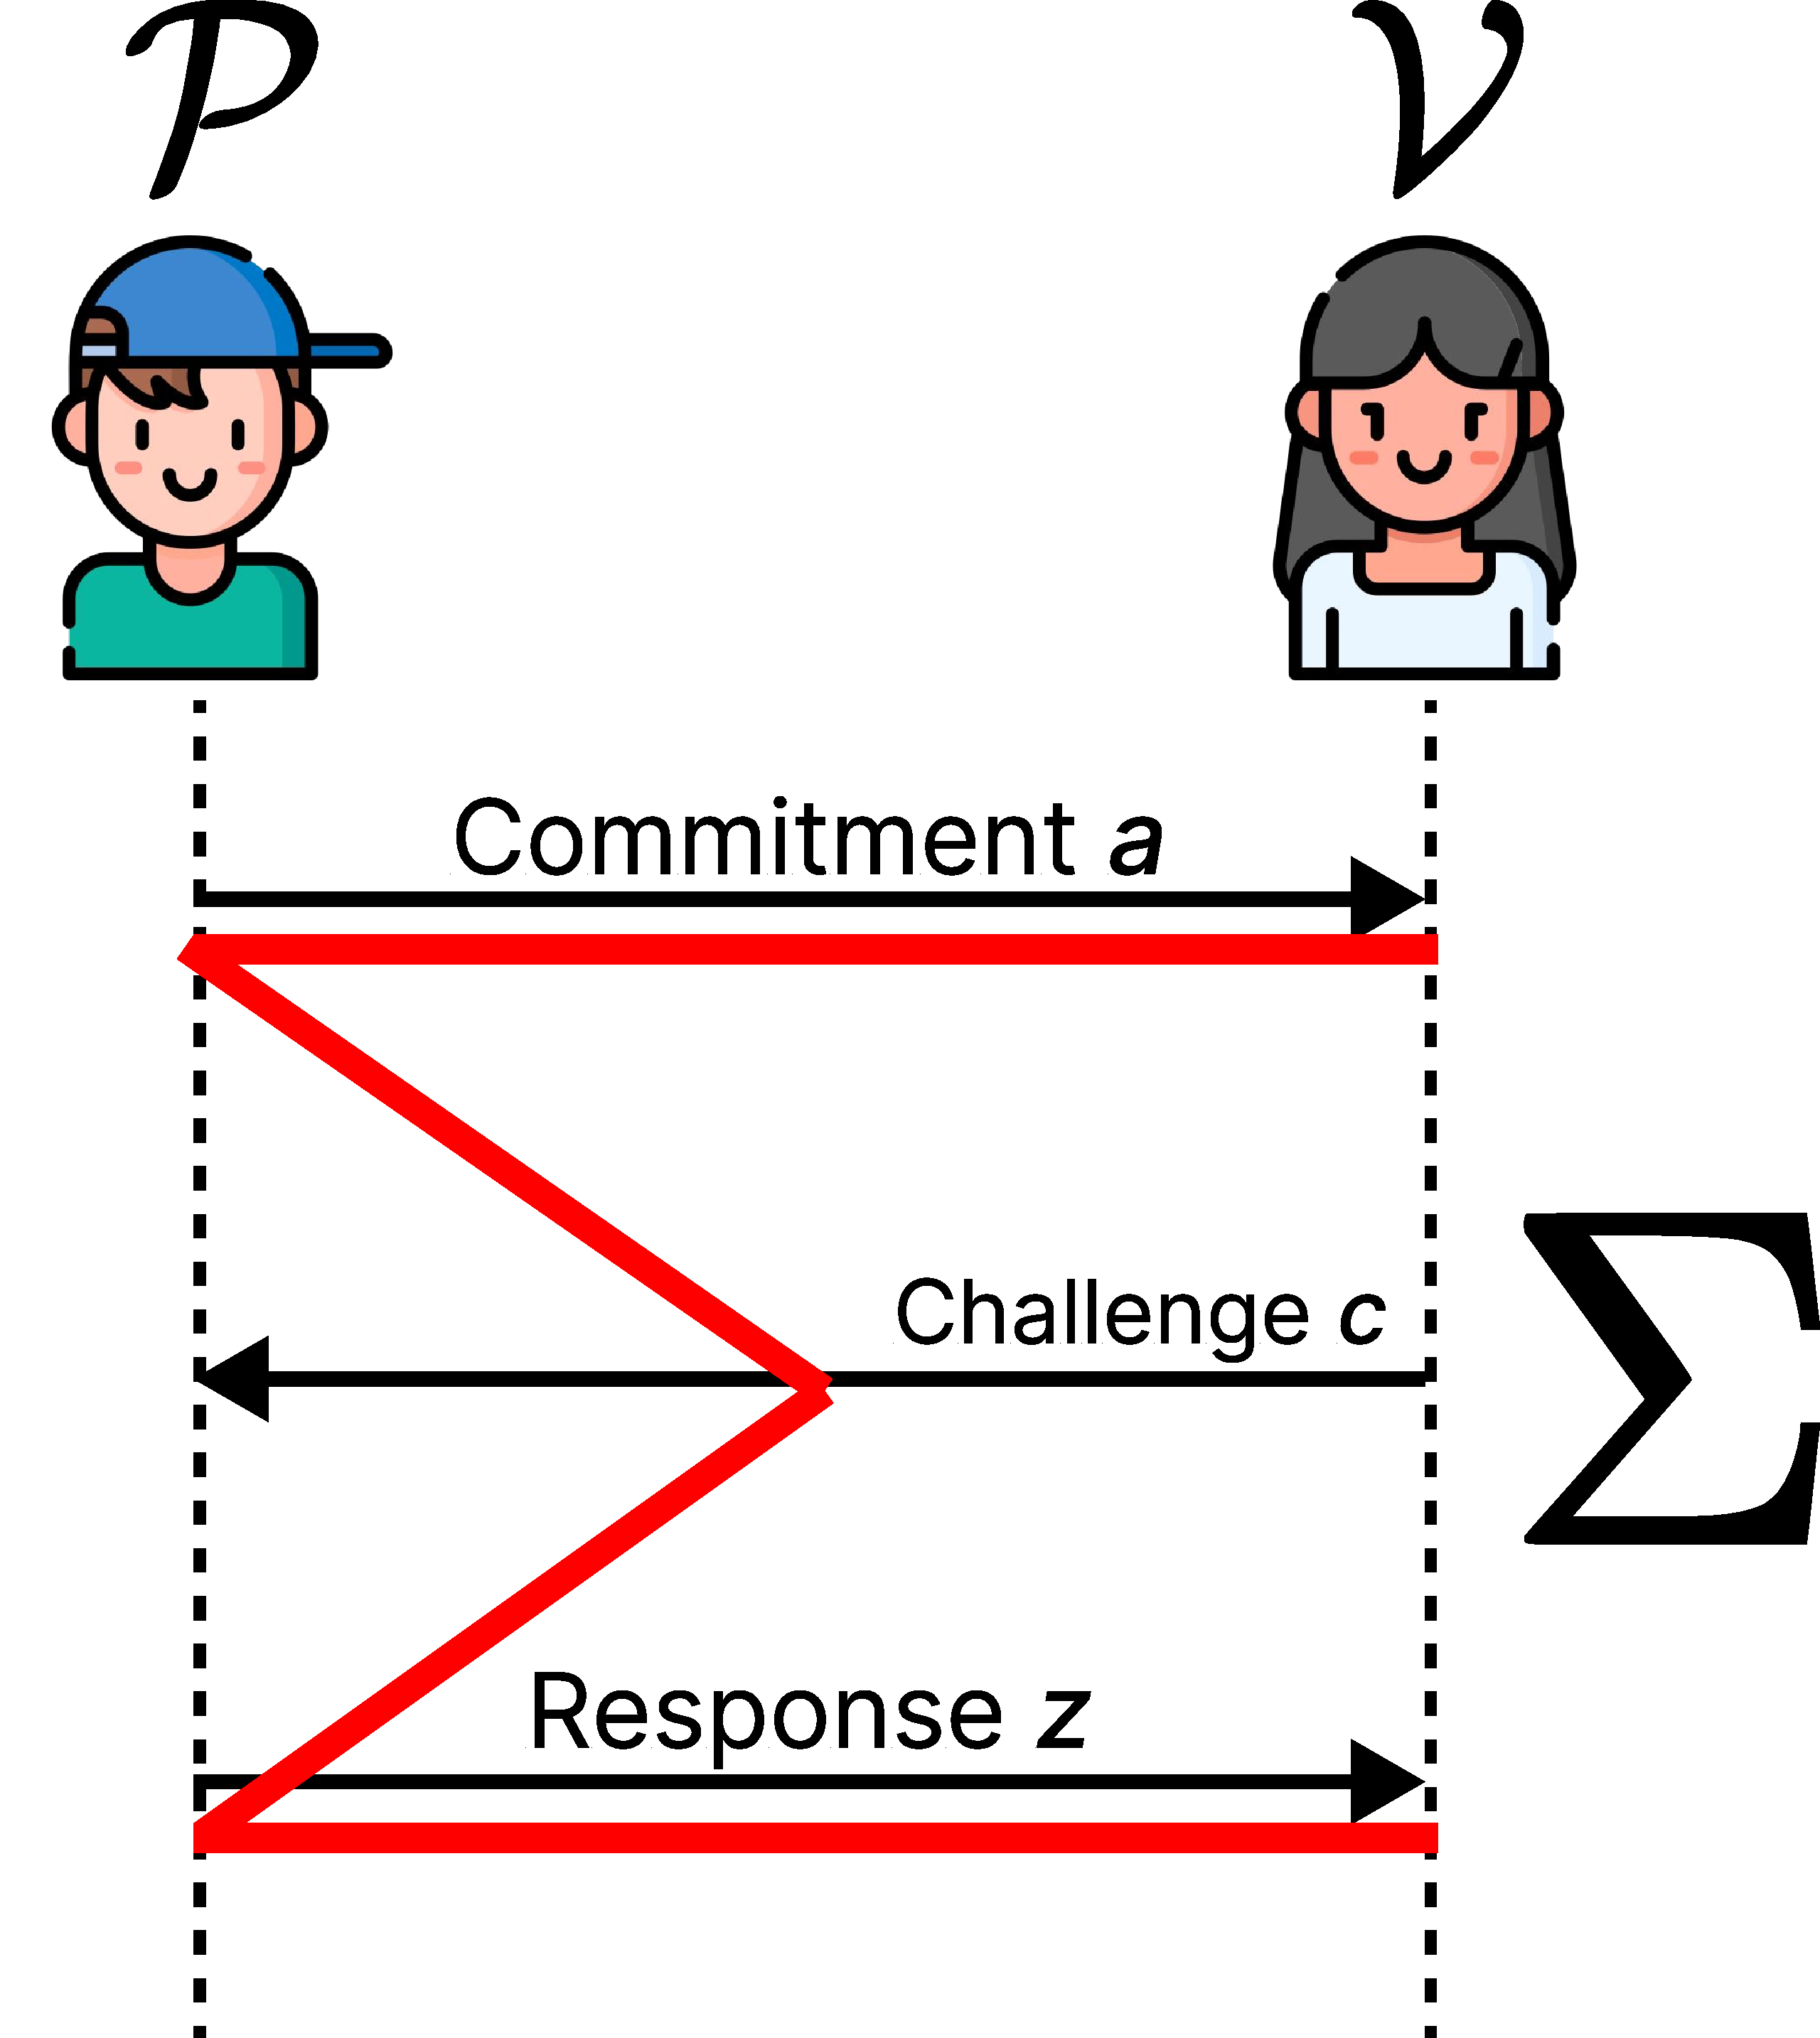
\includegraphics[width=0.5\textwidth]{images/lecture_7/sigma_protocol_illustration.pdf}
            \caption{Why $\Sigma$-protocols are called so.}
        \end{figure}
    \end{frame}

    \begin{frame}{Special Soundness}
        \begin{definition}[Special Soundness]
            Let $(\mathcal{P}, \mathcal{V})$ be a $\Sigma$-protocol for $\mathcal{R} \subseteq \mathcal{X} \times \mathcal{Y}$. We that that $(\mathcal{P},\mathcal{V})$ is \textbf{special sound} if there exists a witness extractor $\mathcal{E}$ such that, given statement $x \in \mathcal{X}$ and two accepting conversations $(a,c,z)$ and $(a,c',z')$ (where $c \neq c'$)\footnote{Notice that initial commitments in both conversations are the same!}, the extractor can always efficiently compute the witness $w$ such that $(x,w) \in \mathcal{R}$.\pause
        \end{definition}

        \begin{example}
            The Schnorr protocol is special sound because, given two accepting conversations $(a,e,\sigma)$ and $(a,e',\sigma')$, we can compute the witness $\alpha$. You can verify that $\alpha = \Delta \sigma / \Delta e$ for $\Delta \sigma = \sigma' - \sigma$ and $\Delta e = e' - e$ suffices.
        \end{example}
    \end{frame}

    \section{Sigma Protocols Examples}
    \subsection{Okamoto Representation Protocol}

    \begin{frame}{Okamoto's Protocol}
        Again, let $\mathbb{G}$ be a cyclic group of prime order $q$ with a generator $g \in \mathbb{G}$ and let $h \in \mathbb{G}$ an arbitrary group element.\pause

        \begin{definition}
            For $u \in \mathbb{G}$, a \textbf{representation} relative to $g$ and $h$ is a pair $(\alpha,\beta) \in \mathbb{Z}_q \times \mathbb{Z}_q$ such that $u=g^{\alpha}h^{\beta}$.\pause
        \end{definition}

        \begin{block}{Remark}
            Notice that for the given $u$ there are exactly $q$ representations relative to $g$ and $h$. Indeed, $\forall \beta \in \mathbb{Z}_q \, \exists! \alpha \in \mathbb{Z}_q: g^{\alpha} = uh^{-\beta}$. \pause
        \end{block}

        \begin{alertblock}{Question}
            How do we actually prove that $\mathcal{P}$ knows the representation of $u$?
            \begin{equation*}
                \mathcal{R} = \left\{ (u,(\alpha,\beta)) \in \mathbb{G} \times \mathbb{Z}_q^2: u = g^{\alpha}h^{\beta} \right\}
            \end{equation*}
        \end{alertblock}
    \end{frame}

    \begin{frame}{Okamoto's Protocol Flow}
        \begin{definition}[Okamoto's Identification Protocol]
            \textbf{Okamoto's Protocol} consists of two algorithms: $(\mathcal{P}, \mathcal{V})$, where the prover is assumed to know $(u,(\alpha,\beta)) \in \mathcal{R}$ defined above. The protocol is defined as follows:\pause
            \begin{enumerate}
                \item $\mathcal{P}$ computes $\alpha_r \xleftarrow{R} \mathbb{Z}_q, \; \beta_r \xleftarrow{R} \mathbb{Z}_q, \; u_r \gets g^{\alpha_r}h^{\beta_r}$ and sends commitment $u_r$ to $\mathcal{V}$.\pause
                \item $\mathcal{V}$ samples the challenge $c \xleftarrow{R} \mathbb{Z}_q$ and sends $c$ to $\mathcal{P}$.\pause
                \item $\mathcal{P}$ computes $\alpha_z \gets \alpha_r + \alpha c, \beta_z \gets \beta_r + \beta c$ and sends $\mathbf{z} = (\alpha_z,\beta_z)$.\pause
                \item $\mathcal{V}$ checks whether $g^{\alpha_z}h^{\beta_z} = u_r u^c$ and accepts or rejects the proof.\pause
            \end{enumerate}
        \end{definition}

        \begin{alertblock}{Announcement}
            We will code the non-interactive Okamoto's protocol in the next section! Stay tuned!
        \end{alertblock}
    \end{frame}

    \begin{frame}{Okamoto's Protocol Correctness}
        \begin{theorem}
            Okamoto's Protocol is a $\Sigma$-protocol for the relation $\mathcal{R}$ which is Honest-Verifier Zero-Knowledge (HVZK).\pause
        \end{theorem}
        
        \textbf{Part of the proof.} Again, let us show \textit{correctness} and \textit{special soundness} without honest-verifier zero-knowledge properties.\pause
        
        \textit{Completeness.} Suppose indeed that $(u,(\alpha,\beta)) \in \mathcal{R}$. Then, the verification condition can be written as follows:\pause
        \begin{equation*}
            g^{\alpha_z}h^{\beta_z} \pause = g^{\alpha_r + \alpha c}h^{\beta_r + \beta c} \pause = g^{\alpha_r}g^{\alpha c}h^{\beta_r}h^{\beta c} \pause = \underbrace{(g^{\alpha_r}h^{\beta_r})}_{=u_r} \cdot (\underbrace{g^{\alpha}h^{\beta}}_{=u})^c \pause = u_r u^c
        \end{equation*}
    \end{frame}

    \begin{frame}{Okamoto's Protocol Special Soundness}
        \textit{Special Soundness}. Suppose we are given two accepting conversations: $(u_r,c,(\alpha_z,\beta_z))$ and $(u_r,c',(\alpha_z',\beta_z'))$ and we want to construct an extractor $\mathcal{E}$ which would give us a witness $(\alpha,\beta)$.\pause In this case, we have the following holding:
        \begin{equation*}
            g^{\alpha_z}h^{\beta_z} = u_r u^c, \; g^{\alpha_z'}h^{\beta_z'} = u_r u^{c'}
        \end{equation*}
        
        \pause We can divide the former by the latter to obtain:
        \begin{equation*}
            g^{\alpha_z - \alpha_z'}h^{\beta_z - \beta_z'} = u^{c-c'} \pause = g^{\textcolor{green!80!black}{\alpha}(c-c')}h^{\textcolor{blue!80!black}{\beta}(c-c')},\pause
        \end{equation*}

        from which the extractor $\mathcal{E}$ can efficiently compute witness as follows: $\textcolor{green!80!black}{\alpha} \gets (\alpha_z - \alpha_z')\big/(c-c')$ and $\textcolor{blue!80!black}{\beta} \gets (\beta_z - \beta_z')\big/(c-c')$.
    \end{frame}

    \subsection{Chaum-Pedersen Protocol}
    \begin{frame}{Diffie-Hellman Triplets}
        Suppose we are given the cyclic group $\mathbb{G}$ or prime order $q$ and generator $g \in \mathbb{G}$. \pause

        \begin{definition}
            A triplet $(u,v,w) \in \mathbb{G}^3$ is a \textbf{Diffie-Hellman triplet} if $\exists \alpha, \beta \in \mathbb{Z}_q: u = g^{\alpha}, v = g^{\beta}, w = g^{\alpha\beta}$.\pause
        \end{definition}

        \begin{block}{Alternative DH-triple Definition}
            $(u,v,w)$ is a DH-triplet iff $\exists \beta \in \mathbb{Z}_q: v = g^{\beta}, w = u^{\beta}$.\pause
        \end{block}

        Now, this makes it easier to define the relation $\mathcal{R}$ for the Chaum-Pedersen protocol:
        \begin{equation*}
            \mathcal{R} = \left\{ ((u,v,w), \beta) \in \mathbb{G}^3 \times \mathbb{Z}_q: v = g^{\beta} \wedge w = u^{\beta} \right\}
        \end{equation*}
    \end{frame}

    \begin{frame}{Chaum-Pedersen Protocol}
        \begin{definition}[Chaum-Pedersen Protocol]
            \textbf{Chaum-Pedersen Protocol} consists of two algorithms: $(\mathcal{P}, \mathcal{V})$, where the prover is assumed to know $(\beta,(u,v,w)) \in \mathcal{R}$ defined above. The protocol is defined as follows:\pause
            \begin{enumerate}
                \item $\mathcal{P}$ computes $\beta_r \xleftarrow{R} \mathbb{Z}_q, \; v_r \xleftarrow{R} g^{\beta_r}, \; w_r \gets u^{\beta_r}$ and sends $(u_r,w_r)$ to $\mathcal{V}$.\pause
                \item $\mathcal{V}$ samples the challenge $c \xleftarrow{R} \mathbb{Z}_q$ and sends $c$ to $\mathcal{P}$.\pause
                \item $\mathcal{P}$ computes $\beta_z \gets \beta_r + \beta c$ and sends $\beta_z$ to $\mathcal{V}$.\pause
                \item $\mathcal{V}$ checks whether two conditions hold: $g^{\beta_z} = v_rv^c$ and $u^{\beta_z} = w_r w^c$, and accepts or rejects the proof accordingly.\pause
            \end{enumerate}
        \end{definition}
        
        \begin{theorem}
            Chaum-Pedersen Protocol is a $\Sigma$-protocol for the relation $\mathcal{R}$ which is Honest-Verifier Zero-Knowledge (HVZK).
        \end{theorem}
    \end{frame}

    \subsection{Pre-image of a homomorphism $\Sigma$-protocol}

    \begin{frame}{Homomorphism-based Sigma Protocol}
        Let us formulate the core objects that we will use in this section:\pause
        \begin{itemize}
            \item $(\mathbb{H}, +)$ is a finite abelian input group.\pause
            \item $(\mathbb{T}, \times)$ is a finite abelian output group.\pause
            \item $\psi: \mathbb{H} \to \mathbb{T}$ is a hard-to-invert homomorphism.\pause
            \item $\mathcal{F} = \mathsf{Hom}(\mathbb{H}, \mathbb{T})$ is a set of all homomorphisms from $\mathbb{H}$ to $\mathbb{T}$.\pause
        \end{itemize}

        \begin{block}{Reminder}
            Homomorphism $\psi: \mathbb{H} \to \mathbb{T}$ is a function, satisfying the following property:
            \begin{equation*}
                \forall h_1, h_2 \in \mathbb{H}: \psi(h_1 + h_2) = \psi(h_1)\psi(h_2)
            \end{equation*}
        \end{block}

        \pause\begin{alertblock}{Note}
            If between input and output we have an easy-to-compute and hard-to-invert homomorphism, we can use Sigma protocols to prove pre-images of this homomorphism!
        \end{alertblock}
    \end{frame}

    \begin{frame}{Problem Statement}
        Define the following relation:
        \begin{equation*}
            \mathcal{R} = \left\{ ((t,\psi), h) \in (\mathbb{T} \times \mathcal{F}) \times \mathbb{H}: \psi(h) = t \right\}
        \end{equation*}

        \pause $\mathcal{P}$ wants to convince $\mathcal{V}$ that he knows witness $h$ to the statement $(t,\psi)$.  \pause
        \begin{example}
            Now, why does this generalize the previous protocols? Well, let us consider all previous examples:
            \begin{itemize}
                \item \textbf{Schnorr Protocol:} Here we have $\mathbb{H} = \mathbb{Z}_q$, $\mathbb{T} = \mathbb{G}$, and $\psi: \mathbb{Z}_q \to \mathbb{G}$ is defined as $\psi(\alpha) = g^{\alpha}$. Moreover, here $\psi$ is an isomorphism!\pause
                \item \textbf{Okamoto Protocol:} Here we have $\mathbb{H} = \mathbb{Z}_q^2$, $\mathbb{T} = \mathbb{G}$, and $\psi: \mathbb{Z}_q^2 \to \mathbb{G}$ is defined as $\psi(\alpha,\beta) = g^{\alpha}h^{\beta}$.\pause
                \item \textbf{Chaum-Pedersen Protocol:} Here we have $\mathbb{H} = \mathbb{Z}_q$, $\mathbb{T} = \mathbb{G}^2$, and $\psi: \mathbb{Z}_q \to \mathbb{G}^2$ is defined as $\psi(\beta) = (g^{\beta},u^{\beta})$. 
            \end{itemize}
        \end{example}
    \end{frame}

    \begin{frame}{Sigma Protocol}
        \begin{definition}[Sigma Protocol for the pre-image of a homomorphism]
            The protocol consists of two algorithms: $(\mathcal{P}, \mathcal{V})$, where the prover is assumed to know the witness $h \in \mathbb{H}$ defined above. The protocol is defined as follows:\pause
            \begin{enumerate}
                \item $\mathcal{P}$ computes $h_r \xleftarrow{R} \mathbb{H}, t_r \gets \psi(h_r) \in \mathbb{T}$ and sends $t_r$ to the verifier $\mathcal{V}$.\pause
                \item $\mathcal{V}$ samples the challenge $c \xleftarrow{R} \mathcal{C} \subset \mathbb{Z}$ from the challenge space and sends $c$ to $\mathcal{P}$.\pause
                \item $\mathcal{P}$ computes $h_z \gets h_r + h\cdot c$ and sends $h_z$ to $\mathcal{V}$.\pause
                \item $\mathcal{V}$ checks whether $\psi(h_z) = t_r t^c$, and accepts or rejects the proof.\pause
            \end{enumerate}
        \end{definition}

        \begin{theorem}
            Such protocol is a $\Sigma$-protocol for the relation $\mathcal{R}$ which is Honest-Verifier Zero-Knowledge (HVZK).
        \end{theorem}
    \end{frame}

    \subsection{Combining $\Sigma$-Protocols}

    \begin{frame}{Combining $\Sigma$-Protocols}
        One of the features (which we are not going to delve into) is the ability to combine $\Sigma$-protocols to prove more complex statements. \pause Namely,
        \begin{itemize}
            \item Given two relations $\mathcal{R}_0$ and $\mathcal{R}_1$, we can prove that the prover knows witnesses for both relations.\pause
            \item Given two relations $\mathcal{R}_0$ and $\mathcal{R}_1$, we can prove that the prover knows a witness for at least one of the relations. \pause
        \end{itemize}

        \begin{example}
            $\mathcal{P}$ can prove that he either knows the discrete log of $u$ or the representation of $u$ relative to $g$ and $h$. Moreover, $\mathcal{V}$ does not know which of the two statements $\mathcal{P}$ is proving.
        \end{example}
    \end{frame}

    \section{Coding Time!}

    \subsection{Okamoto's Protocol}
    \begin{frame}{Methodology}
        \begin{block}{Reminder}
            Suppose prover had messages $(m_1,m_2,\dots,m_n)$ before verifier sends a challenge $c$. If $x$ is a public statement, it suffices to choose $c \gets H(x,m_1,\dots,m_n)$ without any interaction.\pause
        \end{block}

        Let us turn \textbf{Okamoto's Protocol} into a non-interactive proof using the Fiat-Shamir heuristic! \pause

        \begin{block}{Reminder: Okamoto's Identification Protocol}
            \begin{enumerate}
                \item $\mathcal{P}$ computes $\alpha_r \xleftarrow{R} \mathbb{Z}_q, \; \beta_r \xleftarrow{R} \mathbb{Z}_q, \; u_r \gets g^{\alpha_r}h^{\beta_r}$ and sends commitment $u_r$ to $\mathcal{V}$.
                \item $\mathcal{V}$ samples the challenge $c \xleftarrow{R} \mathbb{Z}_q$ and sends $c$ to $\mathcal{P}$.
                \item $\mathcal{P}$ computes $\alpha_z \gets \alpha_r + \alpha c, \beta_z \gets \beta_r + \beta c$ and sends $\mathbf{z} = (\alpha_z,\beta_z)$.
                \item $\mathcal{V}$ checks whether $g^{\alpha_z}h^{\beta_z} = u_r u^c$ and accepts or rejects the proof.
            \end{enumerate}
        \end{block}
    \end{frame}

    \begin{frame}{Non-Interactive Okamoto Protocol}
        \begin{block}{Okamoto's Non-Interactive Identification Protocol}
            Now, we apply the \textit{Fiat-Shamir Transformation}.
            \begin{itemize}
                \item $\mathsf{Prove}(1^{\lambda})$: On input $(u,(\alpha,\beta)) \in \mathbb{G} \times \mathbb{Z}_q^2$, 
                \begin{enumerate}
                    \item Sample $\alpha_r,\beta_r \xleftarrow{R} \mathbb{Z}_q$ and compute $u_r \gets g^{\alpha_r}h^{\beta_r}$.
                    \item Using the hash function $H: \mathbb{G} \times \mathbb{G} \to \mathcal{C}$, compute $c \gets H(u,u_r)$.
                    \item Compute $\alpha_z \gets \alpha_r + \alpha c, \beta_z \gets \beta_r + \beta c$ and publish $(u_r,\alpha_z,\beta_z)$ as a proof $\pi$.
                \end{enumerate}
                \item $\mathsf{Verify}$: Upon receiving statement $u$ and a proof $\pi=(u_r,\alpha_z,\beta_z)$, the verifier:
                \begin{enumerate}
                    \item Recomputes the challenge $c$ using the hash function.
                    \item Accepts if and only if $g^{\alpha_z}h^{\beta_z} = u_ru^c$.
                \end{enumerate}
            \end{itemize}
        \end{block}
    \end{frame}

    \begin{frame}{Non-Interactive Okamoto Protocol}
        \begin{block}{Okamoto's Non-Interactive Identification Protocol}
            Now, we apply the \textit{Fiat-Shamir Transformation}.
        \end{block}
    \end{frame}

    \begin{frame}{Non-Interactive Okamoto Protocol}
        \begin{block}{Okamoto's Non-Interactive Identification Protocol}
            Now, we apply the \textit{Fiat-Shamir Transformation}.
            \begin{itemize}
                \item \textcolor{blue!80!black}{$\mathsf{Prove}(1^{\lambda})$: On input $(u,(\alpha,\beta)) \in \mathbb{G} \times \mathbb{Z}_q^2$, }
            \end{itemize}
        \end{block}
    \end{frame}

    \begin{frame}{Non-Interactive Okamoto Protocol}
        \begin{block}{Okamoto's Non-Interactive Identification Protocol}
            Now, we apply the \textit{Fiat-Shamir Transformation}.
            \begin{itemize}
                \item \textcolor{gray}{$\mathsf{Prove}(1^{\lambda})$: On input $(u,(\alpha,\beta)) \in \mathbb{G} \times \mathbb{Z}_q^2$, }
                \begin{enumerate}
                    \item \textcolor{blue!80!black}{Sample $\alpha_r,\beta_r \xleftarrow{R} \mathbb{Z}_q$ and compute $u_r \gets g^{\alpha_r}h^{\beta_r}$.}
                \end{enumerate}
            \end{itemize}
        \end{block}
    \end{frame}

    \begin{frame}{Non-Interactive Okamoto Protocol}
        \begin{block}{Okamoto's Non-Interactive Identification Protocol}
            \textcolor{gray}{Now, we apply the \textit{Fiat-Shamir Transformation}.}
            \begin{itemize}
                \item \textcolor{gray}{$\mathsf{Prove}(1^{\lambda})$: On input $(u,(\alpha,\beta)) \in \mathbb{G} \times \mathbb{Z}_q^2$, }
                \begin{enumerate}
                    \item \textcolor{gray}{Sample $\alpha_r,\beta_r \xleftarrow{R} \mathbb{Z}_q$ and compute $u_r \gets g^{\alpha_r}h^{\beta_r}$.}
                    \item \textcolor{blue!80!black}{Using the hash function $H: \mathbb{G} \times \mathbb{G} \to \mathcal{C}$, compute $c \gets H(u,u_r)$.}
                \end{enumerate}
            \end{itemize}
        \end{block}
    \end{frame}

    \begin{frame}{Non-Interactive Okamoto Protocol}
        \begin{block}{Okamoto's Non-Interactive Identification Protocol}
            \textcolor{gray}{Now, we apply the \textit{Fiat-Shamir Transformation}.}
            \begin{itemize}
                \item \textcolor{gray}{$\mathsf{Prove}(1^{\lambda})$: On input $(u,(\alpha,\beta)) \in \mathbb{G} \times \mathbb{Z}_q^2$, }
                \begin{enumerate}
                    \item \textcolor{gray}{Sample $\alpha_r,\beta_r \xleftarrow{R} \mathbb{Z}_q$ and compute $u_r \gets g^{\alpha_r}h^{\beta_r}$.}
                    \item \textcolor{gray}{Using the hash function $H: \mathbb{G} \times \mathbb{G} \to \mathcal{C}$, compute $c \gets H(u,u_r)$.}
                    \item \textcolor{blue!80!black}{Compute $\alpha_z \gets \alpha_r + \alpha c, \beta_z \gets \beta_r + \beta c$ and publish $(u_r,\alpha_z,\beta_z)$ as a proof $\pi$.}
                \end{enumerate}
            \end{itemize}
        \end{block}
    \end{frame}

    \begin{frame}{Non-Interactive Okamoto Protocol}
        \begin{block}{Okamoto's Non-Interactive Identification Protocol}
            \textcolor{gray}{Now, we apply the \textit{Fiat-Shamir Transformation}.}
            \begin{itemize}
                \item \textcolor{gray}{$\mathsf{Prove}(1^{\lambda})$: On input $(u,(\alpha,\beta)) \in \mathbb{G} \times \mathbb{Z}_q^2$, }
                \begin{enumerate}
                    \item \textcolor{gray}{Sample $\alpha_r,\beta_r \xleftarrow{R} \mathbb{Z}_q$ and compute $u_r \gets g^{\alpha_r}h^{\beta_r}$.}
                    \item \textcolor{gray}{Using the hash function $H: \mathbb{G} \times \mathbb{G} \to \mathcal{C}$, compute $c \gets H(u,u_r)$.}
                    \item \textcolor{gray}{Compute $\alpha_z \gets \alpha_r + \alpha c, \beta_z \gets \beta_r + \beta c$ and publish $(u_r,\alpha_z,\beta_z)$ as a proof $\pi$.}
                \end{enumerate}
                \item \textcolor{blue!80!black}{$\mathsf{Verify}$: Upon receiving statement $u$ and a proof $\pi=(u_r,\alpha_z,\beta_z)$, the verifier:}
            \end{itemize}
        \end{block}
    \end{frame}

    \begin{frame}{Non-Interactive Okamoto Protocol}
        \begin{block}{Okamoto's Non-Interactive Identification Protocol}
            \textcolor{gray}{Now, we apply the \textit{Fiat-Shamir Transformation}.}
            \begin{itemize}
                \item \textcolor{gray}{$\mathsf{Prove}(1^{\lambda})$: On input $(u,(\alpha,\beta)) \in \mathbb{G} \times \mathbb{Z}_q^2$, }
                \begin{enumerate}
                    \item \textcolor{gray}{Sample $\alpha_r,\beta_r \xleftarrow{R} \mathbb{Z}_q$ and compute $u_r \gets g^{\alpha_r}h^{\beta_r}$.}
                    \item \textcolor{gray}{Using the hash function $H: \mathbb{G} \times \mathbb{G} \to \mathcal{C}$, compute $c \gets H(u,u_r)$.}
                    \item \textcolor{gray}{Compute $\alpha_z \gets \alpha_r + \alpha c, \beta_z \gets \beta_r + \beta c$ and publish $(u_r,\alpha_z,\beta_z)$ as a proof $\pi$.}
                \end{enumerate}
                \item \textcolor{gray}{$\mathsf{Verify}$: Upon receiving statement $u$ and a proof $\pi=(u_r,\alpha_z,\beta_z)$, the verifier:}
                \begin{enumerate}
                    \item \textcolor{blue!80!black}{Recomputes the challenge $c$ using the hash function.}
                \end{enumerate}
            \end{itemize}
        \end{block}
    \end{frame}

    \begin{frame}{Non-Interactive Okamoto Protocol}
        \begin{block}{Okamoto's Non-Interactive Identification Protocol}
            \textcolor{gray}{Now, we apply the \textit{Fiat-Shamir Transformation}.}
            \begin{itemize}
                \item \textcolor{gray}{$\mathsf{Prove}(1^{\lambda})$: On input $(u,(\alpha,\beta)) \in \mathbb{G} \times \mathbb{Z}_q^2$, }
                \begin{enumerate}
                    \item \textcolor{gray}{Sample $\alpha_r,\beta_r \xleftarrow{R} \mathbb{Z}_q$ and compute $u_r \gets g^{\alpha_r}h^{\beta_r}$.}
                    \item \textcolor{gray}{Using the hash function $H: \mathbb{G} \times \mathbb{G} \to \mathcal{C}$, compute $c \gets H(u,u_r)$.}
                    \item \textcolor{gray}{Compute $\alpha_z \gets \alpha_r + \alpha c, \beta_z \gets \beta_r + \beta c$ and publish $(u_r,\alpha_z,\beta_z)$ as a proof $\pi$.}
                \end{enumerate}
                \item \textcolor{gray}{$\mathsf{Verify}$: Upon receiving statement $u$ and a proof $\pi=(u_r,\alpha_z,\beta_z)$, the verifier:}
                \begin{enumerate}
                    \item \textcolor{gray}{Recomputes the challenge $c$ using the hash function.}
                    \item \textcolor{blue!80!black}{Accepts if and only if $g^{\alpha_z}h^{\beta_z} = u_ru^c$.}
                \end{enumerate}
            \end{itemize}
        \end{block}
    \end{frame}

    \begin{frame}{Non-Interactive Okamoto Protocol}
        \begin{block}{Okamoto's Non-Interactive Identification Protocol}
            \textcolor{green!60!black}{Now, we apply the \textit{Fiat-Shamir Transformation}.}
            \begin{itemize}
                \item \textcolor{green!60!black}{$\mathsf{Prove}(1^{\lambda})$: On input $(u,(\alpha,\beta)) \in \mathbb{G} \times \mathbb{Z}_q^2$, }
                \begin{enumerate}
                    \item \textcolor{green!60!black}{Sample $\alpha_r,\beta_r \xleftarrow{R} \mathbb{Z}_q$ and compute $u_r \gets g^{\alpha_r}h^{\beta_r}$.}
                    \item \textcolor{green!60!black}{Using the hash function $H: \mathbb{G} \times \mathbb{G} \to \mathcal{C}$, compute $c \gets H(u,u_r)$.}
                    \item \textcolor{green!60!black}{Compute $\alpha_z \gets \alpha_r + \alpha c, \beta_z \gets \beta_r + \beta c$ and publish $(u_r,\alpha_z,\beta_z)$ as a proof $\pi$.}
                \end{enumerate}
                \item \textcolor{green!60!black}{$\mathsf{Verify}$: Upon receiving statement $u$ and a proof $\pi=(u_r,\alpha_z,\beta_z)$, the verifier:}
                \begin{enumerate}
                    \item \textcolor{green!60!black}{Recomputes the challenge $c$ using the hash function.}
                    \item \textcolor{green!60!black}{Accepts if and only if $g^{\alpha_z}h^{\beta_z} = u_ru^c$.}
                \end{enumerate}
            \end{itemize}
        \end{block}
    \end{frame}

	\begin{frame}{}
      \centering \Large
      \textbf{Thank you for your attention!}
    \end{frame}
\end{document}